\documentclass[a4paper]{article}
\usepackage[english]{babel} 
\usepackage[utf8]{inputenc} 

\usepackage{amssymb,amsmath}
\usepackage{enumerate}
\usepackage{enumitem}

\usepackage{graphicx}
\usepackage{color,soul}
\usepackage{xcolor}

\definecolor{mygreen}{rgb}{0,0.6,0}
\definecolor{mygray}{rgb}{0.5,0.5,0.5}
\definecolor{mymauve}{rgb}{0.58,0,0.82}
\definecolor{greenish}{RGB}{105,114,41}

\usepackage[nottoc,numbib]{tocbibind}

\usepackage{xspace}

\usepackage{tikz}
\usetikzlibrary{arrows, automata}

\usepackage{parskip}

\usepackage{lmodern}

\usepackage[
	pdftex,
	pdfauthor={\@author},
	pdftitle={\@title},
	pdfsubject={},
	pdfkeywords={},
	pdfproducer={},
	pdfcreator={}
]{hyperref}
\hypersetup{
	colorlinks,
	linkcolor={red!50!black},
	citecolor={blue!50!black},
	urlcolor={blue!80!black}
}

\usepackage{pgfgantt}
\usepackage{lscape}

\usepackage{listings}

\lstset{
	backgroundcolor=\color{white},   % choose the background color; you must add \usepackage{color} or \usepackage{xcolor}; should come as last argument
	basicstyle=\ttfamily,        % the size of the fonts that are used for the code
	breakatwhitespace=true,          % sets if automatic breaks should only happen at whitespace
	breaklines=true,                 % sets automatic line breaking
	captionpos=b,                    % sets the caption-position to bottom
	commentstyle=\color{mygreen},    % comment style
	frame=single,	                 % adds a frame around the code
	keepspaces=true,                 % keeps spaces in text, useful for keeping indentation of code (possibly needs columns=flexible)
	columns=flexible,
	keywordstyle=\color{blue},   	 % keyword style
	commentstyle=\color{red},
	language=bash,                   % the language of the code
%	numbers=left,                    % where to put the line-numbers; possible values are (none, left, right)
%	numbersep=5pt,                   % how far the line-numbers are from the code
%	numberstyle=\tiny\color{mygray}, % the style that is used for the line-numbers
	rulecolor=\color{black},         % if not set, the frame-color may be changed on line-breaks within not-black text (e.g. comments (green here))
	showstringspaces=false,
	numberstyle=\small,
	stepnumber=1,                    % the step between two line-numbers. If it's 1, each line will be numbered
	stringstyle=\color{mymauve},     % string literal style
	tabsize=2,	                     % sets default tabsize to 2 spaces
	title=\lstname,                  % show the filename of files included with \lstinputlisting; also try caption instead of title
	morekeywords={match, where, return, --}
}

\newcommand{\lstlistshow}[2]{
	\begin{minipage}{\linewidth}
		\lstinputlisting[language=Dockerfile, caption={#2}]{#1}
	\end{minipage}
}

\newcommand{\lstlistdiscuss}[4]{
	\begin{minipage}{\linewidth}
		\lstinputlisting[language=Dockerfile, numbers=left, firstnumber=#2, linerange={#2-#3}, caption={#4}]{#1}
	\end{minipage}
}

\author{Claudio Bonesana}

\title{
	\begin{center}
		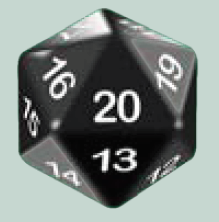
\includegraphics[width=0.4\textwidth]{dice.png}
    \end{center}
    \Large New Techno War \\
	\rule{10cm}{0.3mm} \\
	\large \textit{Installation Guide} \\
}

\date{Last revision: \today}

\setlength\parindent{0pt}


\begin{document}
	
	\maketitle
	
	% \tableofcontents

	% ---------------------------------------------------------------------------------------------------------

	\section{Introduction}

	In this document we are going to explain how to install a development instance of this software and how to deploy a Docker container with the online version of this software.

	\subsection{The project}

	The \textit{"New Techno War"} aims to develop intelligent agents that are capable of play a turn based board game, where different war scenarios are presented. The challenge offered by this game is a dynamic evolution of the game where both attacker and defender need to adapt their strategies to win a scenario.

	If you landed on this page, you will already know everything regarding this project.

	\subsection{Partners}

	This project was developed by \textit{IDSIA} (the Dalle Molle Institute for Studies on Artificial Intelligence) in collaboration with Armasuisse. The board game is produced and developed by Helvetia Games AG.

	% ---------------------------------------------------------------------------------------------------------

	\section{Folder structures}

	This project has two main folders: a \texttt{code} folder and a \texttt{docs} folder.

	In the root folder there are the files used to build the \textbf{Docker} images.

	All documentation files, like this document, and the source files needed to generate the \LaTeX -based documents are stored in the \texttt{docs} folder.
	
	The folder \texttt{code} contains all the source code of the software. This folder is structured as a Python package. In the file \texttt{requirements.txt} it is possible to find a list of all the libraries and packages required to use this software. The code is structured as following:

	\begin{itemize}
		\item \texttt{core} package contains all the scripts required to run the basic game;
		\item \texttt{gui} package contains all the code needed to run the Graphical User Interface (GUI); and
		\item \texttt{utils} package contains some utility scripts and libraries.
	\end{itemize}

	% ---------------------------------------------------------------------------------------------------------

	\section{Technologies}

	The project is entirely written in \texttt{Python 3.7.1}. It uses very basics libraries like \texttt{NumPy} and \texttt{Pandas}.

	For the GUI, we used Flask and Gunicorn. The GUI is realized with templates written in HTML and the interactive part is guaranteed by JavaScript with the help o the JQuery library.

	% ---------------------------------------------------------------------------------------------------------

	\section{Development Environment}

	It is highly recommended to use a Python virtual environment such as \textbf{Anaconda} or \textbf{virtualenv} to manage this project.
	
	From the inside the \texttt{code} folder, it is possible to install all the required packages with

	\begin{lstlisting}
pip install -r requirements.txt\end{lstlisting}

	\section{Local instance}

	A local instance of this software can be run in two different ways.
	
	\subsection{Main Program}
	
	It is possible to execute the \texttt{main.py} program with the following command:
	
	\begin{lstlisting}
python main.py\end{lstlisting}

	It is also possible to change the settings of the game in the lines 27-34 of the \texttt{main.py} file in order to change the played game.

	\subsection{GUI}

	There are different ways to run the GUI program. The simplest way is to execute the \texttt{run.py} script:

	\begin{lstlisting}
python run.py\end{lstlisting}

	or

	\begin{lstlisting}
python.exe -m flask run --port 5000 --host localhost\end{lstlisting}

	Both commands will execute the Flask server in a local instance that is reachable at the address \href{http://localhost:5000/}{http://localhost:5000/}.

	% ---------------------------------------------------------------------------------------------------------

	\section{Docker}

	The whole software is packaged in a \href{https://www.docker.com/}{Docker} image. it is also possible to deploy the software using the included \texttt{docker-compose} file.

	The \texttt{ntw.conf} file is a reverse-proxy configuration for \texttt{Nginx}, used by us to deploy to one of our remote servers.

\end{document}